\documentclass[unknownkeysallowed,xcolor=table]{beamer}
 
\usepackage [T2A,T1] {fontenc}
\usepackage[utf8]{inputenc}
\usepackage[english,russian]{babel}
\usepackage{amsmath}
\usepackage{pifont}
\usepackage{listings}
\usepackage{url}
\usepackage{textcomp}
\usepackage{multirow}
\usepackage{tabulary}

\newcommand{\cmark}{\ding{51}}
\newcommand{\xmark}{\ding{55}}

% to not copy line numbers
\usepackage{accsupp}
% to not copy line numbers

% to not copy line numbers
\newcommand{\noncopynumber}[1]{%
  \BeginAccSupp{method=escape,ActualText={}}%
    \color{blue} #1%
  \EndAccSupp{}%
}
% to not copy line numbers

\setbeamertemplate{navigation symbols}{}

\newcommand{\textapprox}{\raisebox{0.5ex}{\texttildelow}}

\colorlet{mygreen}{green!60!blue}
\colorlet{mymauve}{red!60!blue}
\definecolor{pblue}{rgb}{0.1, 0.2, 0.8}

\newcommand{\rarr}{$\rightarrow$}

\lstset{
      basicstyle=\ttfamily\small,
      commentstyle=\color{mygreen},
      keywordstyle=\color{blue},
%      numberstyle=\tiny\color{blue},
      numberstyle=\noncopynumber,
      stringstyle=\color{mymauve},
      numbers=left,
      stepnumber=1,
      columns=fullflexible,
      breaklines=true,
      postbreak=\mbox{\textcolor{red}{\ensuremath{\hookrightarrow}\space}},
      literate={~} {\textapprox}{1},
      language={[11]C++}
}

\makeatletter
\newcommand{\srcmediumsize}{\@setfontsize{\srcmediumsize}{7pt}{7pt}}
\makeatother

\makeatletter
\newcommand{\srcbigsize}{\@setfontsize{\srcbigsize}{8pt}{8pt}}
\makeatother

\makeatletter
\newcommand{\srcsize}{\@setfontsize{\srcsize}{6pt}{6pt}}
\makeatother

\makeatletter
\newcommand{\srcsmallsize}{\@setfontsize{\srcsmallsize}{5pt}{5pt}}
\makeatother

\title[C++]
{Программирование на языке C++}
 
\subtitle{Вводный курс}
 
\author[А.~Б.~Морозов]
{
  \texorpdfstring{Александр Морозов\newline\href{mailto:gelu.speculum@gmail.com}{gelu.speculum@gmail.com}}
  {Александр Морозов}
}
  
\date[ITMO 2020]
{ИТМО, весенний семестр 2020}
 
\logo{%
  \makebox[0.97\paperwidth]{%
    
\includegraphics[align=c,width=2cm,keepaspectratio]{itmo_logo.png}
    \hfill
    
\includegraphics[align=c,width=1.5cm,keepaspectratio]{itiviti_logo.png}
  }
}

\AtBeginSection[]
{
  \begin{frame}
    \frametitle{Содержание}
    \tableofcontents[currentsection]
  \end{frame}
}

\begin{document}

\frame{\titlepage}

%-------------------------------------------------

\section{Исключения}

\begin{frame}{Исключения}
    \center
    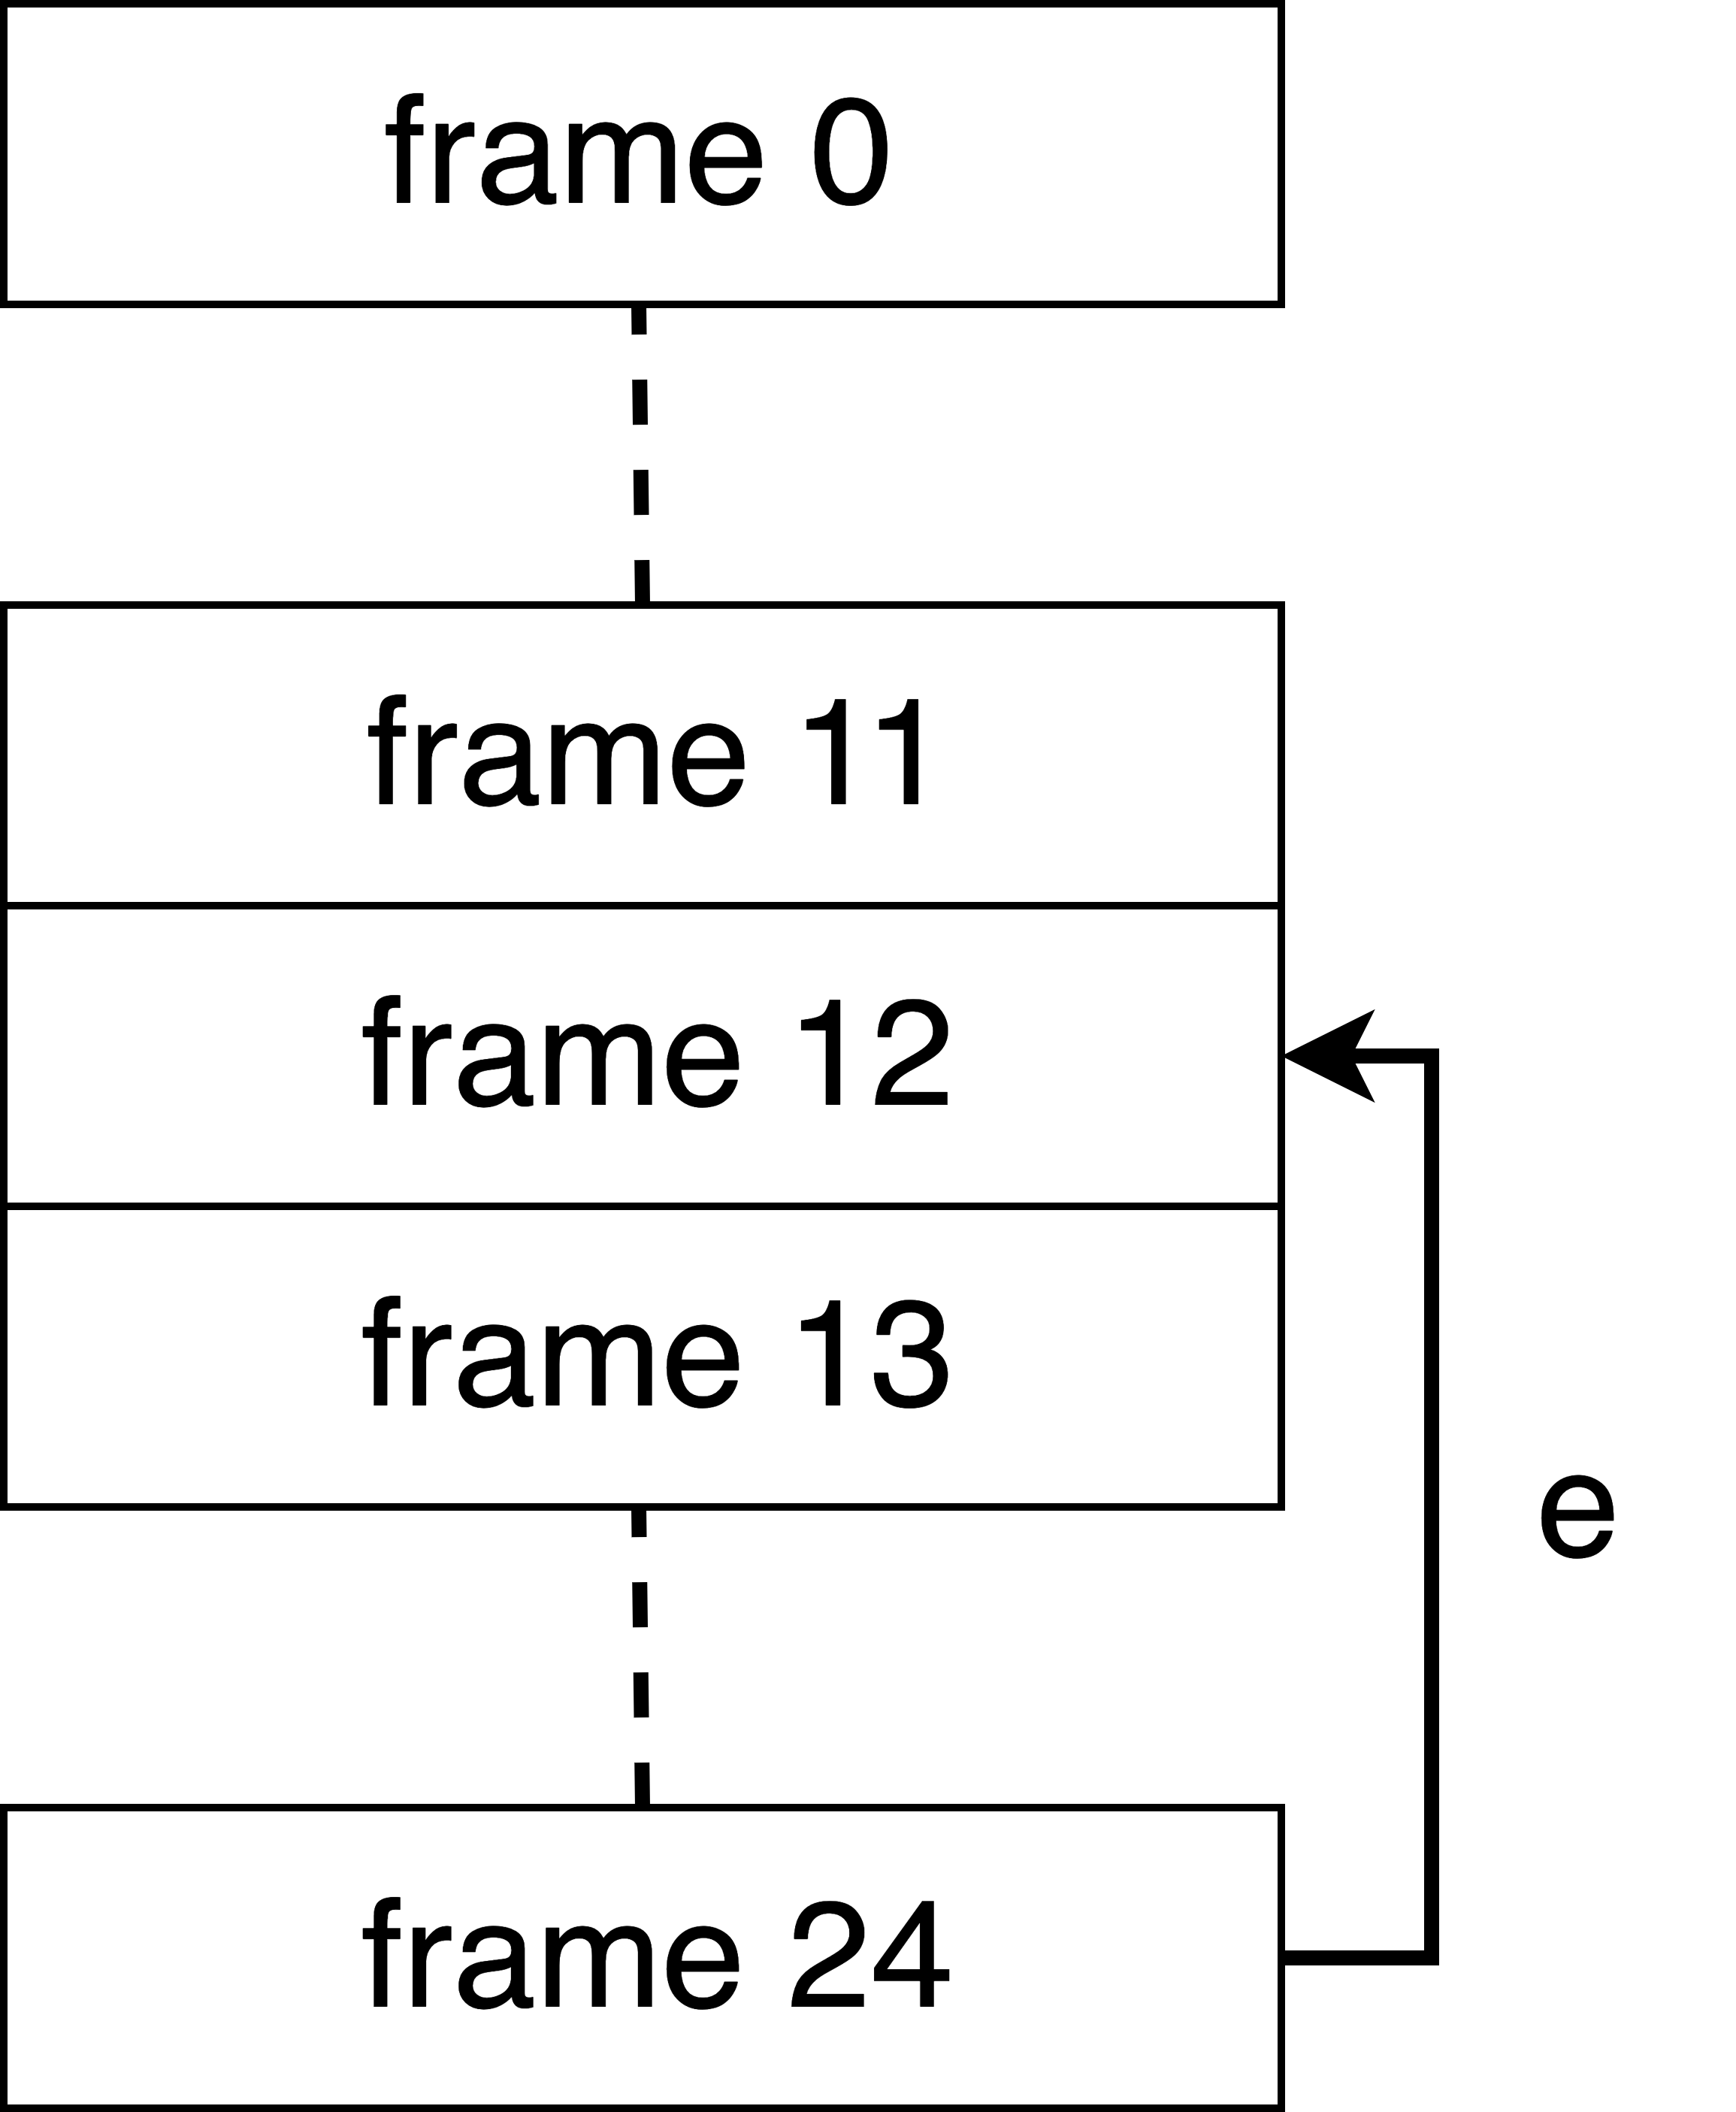
\includegraphics[align=c,width=5cm,keepaspectratio]{images/exception.png}
\end{frame}

\begin{frame}{Для чего используются исключения}
  Функция не может:
  \begin{itemize}
    \item удовлетворить предусловие вызова другой функции, являющейся очередным шагом логики данной \vspace{1em}
    \item удовлетворить постусловие своей работы \vspace{1em}
    \item обеспечить сохранение инварианта, за который она ответственна
  \end{itemize}
\end{frame}

\begin{frame}{Доступные механизмы уведомления вызывающий код об ошибках}
  \begin{itemize}
    \item коды возврата:
      \begin{itemize}
        \item функция имеет возвращаемое значение и резервирует специальное значение(я) для индикации ошибок \vspace{0.5em}
        \item функция имеет среди аргументов те, через которые может передать в вызывающий код индикацию ошибок \vspace{0.5em}
        \item функция использует глобальные переменные для индикации ошибок \vspace{1em}
      \end{itemize}
    \item исключения
  \end{itemize}
\end{frame}

\begin{frame}[fragile]{Пример исключения}
  \begin{lstlisting}[basicstyle=\ttfamily\srcbigsize]
  template <class T>
  class PoolAllocator
  {
  public:
      T * allocate()
      {
          if (/* no space in this pool */) {
              throw std::bad_alloc{};
          }
      }
  };

  void append(const X & x, std::vector<X, PoolAllocator<X>> & v)
  {
      try {
          v.push_back(x);
      }
      catch (const std::bad_alloc & e) {
          // report?
      }
  }
  \end{lstlisting}
\end{frame}

\begin{frame}{\lstinline{throw}}
  \begin{enumerate}
    \item \lstinline{throw} \emph{выражение}
    \item \lstinline{throw}
  \end{enumerate}

  \vspace{1em}

  \begin{enumerate}
    \item Из \emph{выражения} конструируется объект исключения
      \begin{itemize}
        \item если выражение задаёт локальный объект с автоматическим размещением, возможен вызов перемещающего вместо копирующего конструктора
        \item возможна NRVO-подобная оптимизация
      \end{itemize}
      затем управление передаётся в ближайший подходящий по типу обработчик исключения
    \item Пере-выбрасывает исключение: если какое-то исключение уже обрабатывается, \lstinline{throw} вызовет выход из текущего обработчика и передачу управления
      ближайшему следующему, уровнем выше, подходящему по типу. Объект исключения заново не создаётся.
  \end{enumerate}
\end{frame}

\begin{frame}[fragile]{\lstinline{try}-\lstinline{catch}}
  \lstinline{try} \emph{блок} \emph{последовательность обработчиков}

  \vspace{1em}

  Обработчик:
  \begin{itemize}
    \item \lstinline{catch ( expr )} \emph{блок}
    \item \lstinline{catch (...)} \emph{блок}
  \end{itemize}

  \vspace{1em}

  \emph{expr} -- не может быть rvalue ссылкой или неполным типом.
\end{frame}

\begin{frame}{Выбор подходящего обработчика}
  \begin{itemize}
    \item в одной \lstinline{try}-\lstinline{catch} инструкции обработчики проверяются последовательно, от первого к последнему
    \item если параметр обработчика объявлен ссылкой на тип \textbf{T}, то объект исключения должен иметь тот же тип, либо тип класса-потомка
    \item если параметр обработчика объявлен указателем на тип \textbf{T}, то объект исключения должен быть указателем на тот же тип или быть указателем, неявно
      приводимым к типу параметра обработчика
    \item иначе тип объекта исключения должен совпадать с типом параметра обработчика или быть его однозначным доступным потомком
    \item \lstinline{catch (...)} перехватывает исключение любого типа
    \item если подходящего обработчика не найдено, то поиск продолжается уровнем выше
    \item если подходящего обработчика не найдено вообще, программа аварийно завершается
  \end{itemize}
\end{frame}

\begin{frame}[fragile]{Пример выбора обработчика}
  \begin{lstlisting}[basicstyle=\ttfamily\srcsmallsize]
    class MyException : public std::exception
    {
    public:
        const char * what() const
        { return "MyException"; }
    };

    void f(int n)
    {
        if (n < 0) {
            throw std::invalid_argument("Argument must be non-negative");
        }
        else {
            throw MyException;
        }
    }

    void g(int n)
    {
        try {
            f(n);
        }
        catch (const std::logic_error & e) {
            std::cerr << e.what() << std::endl;
        }
    }

    int main()
    {
        try {
            g(-1);
            g(1);
        }
        catch (std::runtime_error e) {
            std::cerr << "Runtime!" << std::endl;
        }
        catch (MyException e) {
            std::cerr << e.what() << std::endl;
        }
    }
  \end{lstlisting}
\end{frame}

\section{Обработка исключений и развёртывание стека}

\begin{frame}{Объект исключения}
  \begin{itemize}
    \item не имеет определённого типа размещения \vspace{1em}
    \item тип = типу выражения в \lstinline{throw}, cv-квалификаторы верхнего уровня отбрасываются \vspace{1em}
    \item является временным объектом, но связывается с lvalue ссылками в параметрах обработчиков \vspace{1em}
    \item существует до выхода из последнего вызванного обработчика, который не перебросил это исключение
  \end{itemize}
\end{frame}

\begin{frame}{Обрабротка исключения}
  В точке выброса исключения нормальное исполнение прерывается и
  \begin{itemize}
    \item производится поиск первого подходящего обработчика -- пока он не найден производится развёртывание стека
    \item в \lstinline{try} блоке инструкции, где найден подходящий обработчик, разрушаются все локальные автоматические переменные в порядке, обратном порядку их
      создания
    \item управление передаётся в найденный обработчик
    \item если выбрасывается другое исключение (до момента вызова обработчика или в процессе его работы), программа аварийно завершается
    \item после завершения блока обработчика, исполнение переходит к следующей за \lstinline{try}-\lstinline{catch} инструкции и восстанавливается нормальное
      исполнение программы
  \end{itemize}
\end{frame}

\begin{frame}{Развёртывание стека}
  Пока развёртывание не дошло до уровня с подходящим обработчиком:
  \begin{itemize}
    \item все автоматические переменные в данной функции разрушаются в порядке, обратном порядку их создания
    \item если текущая функция -- конструктор или деструктор класса, то также разрушаются все полностью сконструированные поля этого объекта
    \item если текущая функция -- делегирующий конструктор класса и делегируемый конструктор успешно завершился, то вызывается деструктор этого класса
    \item если текущая функция -- конструктор, вызванный в рамках \lstinline{new}, то также вызывается освобождение выделенной памяти
    \item исполнение текущей функции полностью завершается и процесс повторяется уровнем выше
  \end{itemize}
\end{frame}

\section{Спецификация исключений и гарантии безопасности}

\begin{frame}{Гарантии безопасности}
  \begin{itemize}
    \item никаких гарантий: после исключения программа оказывается в некорректном состоянии \vspace{1em}
    \item базовая гарантия: программа находится в валидном, но неопределённом состоянии \vspace{1em}
    \item строгая гарантия: состояние программы корректно и возвращено к состоянию до вызова функции, в которой произошло исключение \vspace{1em}
    \item гарантия отсутствия исключений: функция не выбрасывает наружу никаких исключений ни при каких условиях
  \end{itemize}
\end{frame}

\begin{frame}{Спецификация исключений}
  Тип функции включает в себя спецификацию исключений:
  \begin{itemize}
    \item либо функция не может приводить к выбросу исключений
    \item либо функция может приводить к выбросу исключений
  \end{itemize}

  \vspace{1em}

  Спецификацию можно задать явно с помощью \lstinline{noexcept} в конце объявления функции.

  \vspace{1em}

  Как и в случае с типом возвращаемого значения, спецификация исключений не участвует в разрешении перегрузки.

  \vspace{1em}

  Функция, имеющая спецификацию ``без выброса исключений'' может вызывать код, выбрасывающий исключения, но если такое исключение выйдет за рамки этой функции, программа
  аварийно завершится.
\end{frame}

\begin{frame}[fragile]{\lstinline{noexcept}}
  Спецификатор \lstinline{noexcept}:
  \begin{itemize}
    \item \lstinline{noexcept( expr )} -- если \emph{expr} вычисляется в \lstinline{true}, то функция не может выбрасывать исключения
    \item \lstinline{noexcept} -- то же, что \lstinline{noexcept(true)}
  \end{itemize}

  \vspace{1em}

  Оператор \lstinline{noexcept( expr )} -- вычисляется на этапе компиляции, результат \lstinline{true}, если выражение не имеет потенциальных исключений.
  \begin{lstlisting}
  void f() noexcept;
  void g() noexcept(sizeof(int) < 8)
  {
  }
  template <class T>
  void h(T && x) noexcept(noexcept(T(std::declval<T>())));
  \end{lstlisting}
\end{frame}

\begin{frame}{Определение спецификации исключений для функции}
  \begin{itemize}
    \item функция может приводить к выбросу исключений, если
      \begin{itemize}
        \item объявлена с \lstinline{noexcept(expr)} и \lstinline{expr} вычисляется в \lstinline{false} \vspace{0.5em}
        \item объявлена без \lstinline{noexcept} и не является
          \begin{itemize}
            \item деструктором, кроме деструкторов класса чьи подобъекты имеют потенциально выбрасывающие деструкторы \vspace{0.5em}
            \item методом класса, сгенерированным автоматически, если только вызов такого метода не может выбросить исключение \vspace{0.5em}
          \end{itemize}
      \end{itemize}
    \item в противном случае функция не может приводить к выбросу исключений
  \end{itemize}
\end{frame}

\begin{frame}{Определение спецификации исключений для выражения}
  Выражение имеет потенциальные исключения, если
  \begin{itemize}
    \item вызывает функцию, которая может выбрасывать исключения \vspace{0.5em}
    \item неявно вызывает такую фукнцию (например, в конце выражения вызывается деструктор временного объекта) \vspace{0.5em}
    \item является \lstinline{throw} выражением \vspace{0.5em}
    \item является \lstinline{dynamic_cast} выражением для полиморфной ссылки \vspace{0.5em}
    \item является \lstinline{typeid} выражением \vspace{0.5em}
    \item содержит в себе подвыражение, имеющее потенциальные исключения
  \end{itemize}
\end{frame}

\section{RAII}

\begin{frame}{RAII}
  \begin{itemize}
    \item время жизни объектов \vspace{0.5em}
    \item автоматическое размещение \vspace{0.5em}
    \item порядок инициализации \vspace{0.5em}
    \item развёртывание стека
  \end{itemize}

  \vspace{1em}

  \begin{itemize}
    \item ресурс связывается с объектом
    \item инициализация объекта $\equiv$ захват ресурса
    \item время жизни объекта $\equiv$ время доступности ресурса
    \item разрушение объекта $\equiv$ освобождение ресурса
  \end{itemize}
\end{frame}

\begin{frame}[fragile]{Умные указатели}
  \begin{lstlisting}
  void bad()
  {
      X * x = new X();
      ...
      delete x;
  }

  void good()
  {
      const auto px = std::make_unique<X>();
      ...
  } // x is implicitly deleted
  \end{lstlisting}
\end{frame}

\begin{frame}[fragile]{Scope guards}
  \begin{lstlisting}
  std::mutex m;

  void bad()
  {
      m.lock();
      ...
      m.unlock();
  }

  void good()
  {
      std::lock_guard<std::mutex> g(m); // implicit lock
      ...
  } // implicit unlock
  \end{lstlisting}
\end{frame}

\begin{frame}{Реализация класса, инкапсулирующего ресурс}
  \begin{itemize}
    \item ресурс захватывается в конструкторе, подготавливается к использованию, выброс исключения, если что-то пошло не так \vspace{1em}
    \item ресурс освобождается в деструкторе, освобождение не должно бросать исключений \vspace{1em}
    \item обычно такой класс не имеет операций копирования \vspace{1em}
    \item можно реализовать передачу владения ресурсом из одного контекста в другой с помощью конструктора перемещения / оператора перемещающего присваивания класса
  \end{itemize}
\end{frame}

\section{Некоторые вопросы безопасности в контексте комплексных объектов}

\begin{frame}[fragile]{Инициализация}
  \begin{lstlisting}
  class X
  {
      A * m_a = nullptr;
      B * m_b = nullptr;
      std::vector<C> m_c;
  public:
      X(std::size_t n, const C & c)
      {
          m_a = new A();
          m_b = new B();
          m_c.resize(n, c);
      }
  };
  \end{lstlisting}
\end{frame}

\begin{frame}[fragile]{Более безопасная инициализация}
  \begin{lstlisting}
  class X
  {
      std::unique_ptr<A> m_a;
      std::unique_ptr<B> m_b;
      std::vector<C> m_c;
  public:
      X(std::size_t n, const C & c)
          : m_a(std::make_unique<A>())
          , m_b(std::make_unique<B>())
          , m_c(n, c)
      {
      }
  };
  \end{lstlisting}
\end{frame}

\begin{frame}[fragile]{Копирование}
  \begin{lstlisting}
  X::X(const X & other)
      : m_a(std::make_unique<A>(*other.m_a))
      , m_b(std::make_unique<B>(*other.m_b))
      , m_c(other.m_c)
  {
  }

  X & X::operator = (const X & other)
  {
      m_a = std::make_unique<A>(*other.m_a);
      m_b = std::make_unique<B>(*other.m_b);
      m_c = other.m_c;
  }
  \end{lstlisting}
\end{frame}

\begin{frame}[fragile]{Более безопасное копирование}
  \begin{lstlisting}
  X & X::operator = (const X & other)
  {
      using std::swap;
      X tmp(other);
      swap(m_a, tmp.m_a);
      swap(m_b, tmp.m_b);
      swap(m_c, tmp.m_c);
  }
  \end{lstlisting}
\end{frame}

\begin{frame}[fragile]{Объединение операторов копирующего и перемещающего присваивания}
  \begin{lstlisting}
  X & X::operator = (X tmp)
  {
      using std::swap;
      swap(m_a, tmp.m_a);
      swap(m_b, tmp.m_b);
      swap(m_c, tmp.m_c);
  }
  \end{lstlisting}
\end{frame}

\begin{frame}[fragile]{Извлечение элемента из коллекции}
  \begin{lstlisting}
  template <class T>
  class Queue
  {
      std::vector<T> m_data;
  public:
      T dequeue()
      {
          using std::swap;
          swap(m_data.front(), m_data.back());
          T res = std::move(m_data.back());
          m_data.pop_back();
          return res;
      }
  };
  \end{lstlisting}
\end{frame}

\begin{frame}[fragile]{Более безопасное извлечение элемента из коллекции}
  \begin{lstlisting}
  template <class T>
  T & Queue<T>::top()
  {
      return m_data.front();
  }

  template <class T>
  void Queue<T>::pop()
  {
      using std::swap;
      swap(m_data.front(), m_data.back());
      m_data.pop_back();
  }
  \end{lstlisting}
\end{frame}

\end{document}
